\documentclass[11pt]{article}
\usepackage[margin=1in]{geometry}
\usepackage{float}
\usepackage{xcolor}

\usepackage{wrapfig}
\usepackage{subcaption}
\usepackage{amsmath, amsthm, amssymb, mathtools}
\usepackage{newpxtext, newpxmath}

\usepackage{physics}

\NewDocumentCommand{\R}{}{\mathbb{R}}

\usepackage{thmtools}

\RenewDocumentCommand{\qedsymbol}{}{$\blacksquare$}

\declaretheorem{theorem}
\declaretheorem{lemma}
\declaretheorem[style=definition]{definition}

\declaretheorem[style=remark]{example}
\declaretheorem[style=remark]{remark}

\usepackage{tikz}
\usetikzlibrary{arrows}
\usetikzlibrary{arrows.meta}

\usepackage[style=alphabetic]{biblatex}
\addbibresource{sources/library.bib}

\tikzset{
    vertex/.style={
        font = \scriptsize,
        fill=blue!20,
        draw,
        circle,
        inner sep=0pt,
        minimum size=20pt,
    },
    edge/.style={}
}

\NewDocumentCommand{\term}{m}{\emph{#1}}

\usepackage{hyperref}

\hypersetup{
    colorlinks,
    citecolor=blue,
    linkcolor=blue,
    filecolor=blue,      
    urlcolor=blue,
}

\title{The Graph Laplacian and Determining the Connectivity of Meshes}
\author{Eli Griffiths}
\date{November 2024}

\directlua{graph = require("graph")}
\directlua{examples = require("data")}

\begin{document}

\maketitle

\begin{abstract}
    Graphs lend themselves naturally to matrices that encode properties such as which vertices are connected to others and how many vertices are connected to a given vertex. These matrix representations allow us to analyze graphs outside of traditional combinatoric approachs by considering their eigenvalues and eigenvectors. Key to our study is the Laplacian matrix representation of a graph. We first show that the eigenvalues of the Laplacian matrix give insight into if every vertex of a graph is connected to each other via some path through edges, and if not how many separate components there are in which this is the case. We then frame this result within the context of of computational geometry and discuss how more advanced problems in computational geometry can be approached with this spectral framework.
\end{abstract}

\section{Introduction}

Graphs at their core encode the concept of connectivity. A graph is simply vertices and edges where vertices are objects or nodes and edges are connections between these vertices. While simple in concept, this means graphs appear in different fields and applications such modeling friend networks on a social media platform, determining flight schedules for optimal transport, model the structure of chemical compounds, and much more.

Graph theory has always been deeply tied to the field of combinatorics. One of the earliest problems in what we now consider graph theory, Euler's famous K\"onigsberg bridge problem, was solved via methods of counting, a fundamental technique in combinatorics \cite{wilson2013combinatorics}.



\section{Background}

We first outline the basic structure of a graph and related definitions that will be used throughout the paper, following the formalism and notation from \cite{diestelGraphTheory2017}. We adopt the notation that $[S]^n$ is the set of all $n$-element sized subsets of $S$.

\begin{definition}[Graph Structure]
    A \term{graph} is a pair $G = (V, E)$ of sets where $E \subseteq [V]^2$. The elements of $V$ are \term{vertices} and the elements of $E$ are \term{edges}. A vertex $v$ is said to be \term{incident} to an edge $e$ if $v \in e$. Two vertices $v_1$ and $v_2$ are \term{adjacent} or \term{neighbors} if $\qty{v_1, v_2} \in E$. We denote $\qty{v_1, v_2} \in E$ by $v_1 \sim v_2$. The \term{set of neighbors} of a vertex $v$ is denoted by $N(v) \coloneq \qty{w \in V : v \sim w}$. The \term{degree} of a vertex $v$ is $\deg(v) \coloneq |N(v)|$. A \term{subgraph} $H$ of $G$, denoted by $H \subseteq G$, is a graph whose vertex and edge sets are subsets of $G$'s.
\end{definition}

\begin{remark}
    Edges importantly are defined here as two element sets and not as ordered pairs. This makes the graph \textit{undirected}. If the graph was to be directed (that is the edges were to be ordered pairs) the further results of this paper would not hold in general and would require more restrictions.
\end{remark}

\begin{figure}
    \centering
    \caption{Two example graphs in the plane}
    \label{fig:graph_visual}
    \begin{subfigure}[t]{0.45\textwidth}
        \centering
        \begin{tikzpicture}[scale=0.8]
            \directlua{graph.graph_tikz(examples.example1)}
        \end{tikzpicture}   
        \caption{A graph with $7$ vertices and $15$ edges}
        \label{fig:basic_graph}
    \end{subfigure}\hfill
    \begin{subfigure}[t]{0.45\textwidth}
        \centering
        \begin{tikzpicture}[scale=0.8]
            \directlua{graph.graph_tikz(examples.example2)}
        \end{tikzpicture}   
        \caption{A graph with $2$ connected components}
        \label{fig:connected_components}
    \end{subfigure}
\end{figure}

For the purposes of this paper, we will assume that every graph has finitely many vertices (and hence finitely many edges). Consider the illustrations of two graphs in Figure \ref{fig:graph_visual}. Notice that they differ in terms of how connected their vertices are to one other. If each vertex was a city and each edge a road, a car driving on \ref{fig:basic_graph} could get to any city, but a car on the outer ring of \ref{fig:connected_components} would be stuck on the outer ring. That is, there is some path that the car can take from any city to any other city in \ref{fig:basic_graph} but not in \ref{fig:connected_components}. We formalize this notion of paths and connectedness as follows.

\begin{definition}[Connectedness]
    A \term{path} is a non-empty graph $P = (V,E)$ where
    \[
        V = \qty{v_0, v_1, \ldots, v_k} \hspace{2cm} E = \qty{\qty{v_0,v_1}, \ldots, \qty{v_{k-1}, v_k}}
    .\]
    A graph $G$ is then \term{connected} if between any two vertices $v_0$ and $v_f$ there exists a path $P \subseteq G$ starting at $v_0$ and ending at $v_f$. A \term{connected component} of a graph is a subgraph $H \subseteq G$ that is connected and is not contained in any larger connected subgraph.
\end{definition}

\begin{definition}
    The \term{adjacency matrix} $A_G$ and \term{degree matrix} $D_G$ of a graph $G$ with $n$ vertices are the $n \times n$ matrices such that
    \begin{align*}
        (A_G)_{ij} = \begin{cases}
            1 & v_i \sim v_j \\
            0 & \text{otherwise}
        \end{cases} & &
        (D_G)_{ij} = \begin{cases}
            \deg(v_i) & i = j \\
            0 & i \neq j
        \end{cases}
    \end{align*}
    If $G$ is understood via context, we simply refer to them as $A$ and $D$.
\end{definition}

\begin{example}
    The adjacency and degree matrices for the graph in Figure \ref{fig:basic_graph} are

    \begin{align*}
        A =    
        \begin{bmatrix}
            \directlua{graph.adj_matrix(examples.example1)}
        \end{bmatrix} & &
        D = \begin{bmatrix}
            \directlua{graph.deg_matrix(examples.example1)}
        \end{bmatrix}
    \end{align*}
\end{example}


\section{A Graph's Spectra}

\begin{definition}
    The \term{Laplacian Matrix} of a graph $G$ is $L_G \coloneq D_G - A_G$. If $G$ is understood via context, we simply refer to it as $L$.
\end{definition}

Notice that since $L$ is the difference of two symmetric matrices it is also symmetric. Therefore we know that it has eigenvalues that are all real. Of importance to us is that amongst these eigenvalues, we are guranteed to have $0$ as an eigenvalue for any Laplacian matrix.

\begin{theorem}
    The Laplacian matrix $L$ of a graph $G$ has $0$ as an eigenvalue.
\end{theorem}

\begin{proof}
    Let $n$ denote the number of vertices in $G$ and take $x \in \R^n$ to be the vector of all $1$'s. By the definition of the Laplacian matrix, we have $L = D - A$. Consider the product $D x$. Since $D$ is a diagonal, the $i^\text{th}$ component will be the $i^\text{th}$ component of $x$ times the $i^\text{th}$ entry along the diagonal of $D$, which by the definition of $D$ gives $(Dx)_i = \deg v_i$. Now consider the $i^\text{th}$ component of the product $Ax$. We can express it as the sum
    \[
        (Ax)_i = \sum_{j=1}^n (A)_{ij} x_j = \sum_{j=1}^n (A_{ij})
    .\]
    This sum is simply adding up the entries of the $i^\text{th}$ row of $A$. Since the entries are only $0$ and $1$, and are only $1$ when $v_i$ is adjacent to another vertex, the sum is $\deg v_i$. Hence $(Ax)_i = \deg v_i$. Thus $Ax = Dx$ from which we have $Lx = (D - A)x = Dx - Ax = 0$. Therefore $0$ is an eigenvalue of $L$.
\end{proof}

While the matrix representation of the graph Laplacian gave us some basic insight, we will be interested in an alternative description of the Laplacian called the \emph{quadratic form} of the Laplacian for our further analysis. One can find the derivation of its quadratic form in \cite{mohar2004graph} but we shall simply state it here.

\begin{theorem}
    Let $L$ be the laplacian matrix of a finite graph $G$ with $n$ vertices. Then for a given vector $x \in \R^n$,
    \[
        x^T L x = \sum_{v_i \sim v_j} (x_i - x_j)^2.
    \]
\end{theorem}

\begin{remark}
    Sometimes the Laplacian matrix is defined as the unique symmetric matrix $L$ with this quadratic form and the matrix definition is then a derived representation \cite{WATKINS199443}. The choice of the name Laplacian can be motivated by the fact the quadratic form encapsulates the same concepts of ''smoothness''. If each component of $x$ was say the temperature of each vertex, the quadratic form penalizes large differences in temperature when undergoing minimization.
\end{remark}

\begin{lemma}
    \label{lem:block_det}
    For a block diagonal matrix $A$ with blocks $A_i$, $\det(A) = \det(A_1) \det(A_2) \cdots \det(A_n)$
\end{lemma}

\begin{lemma}
    \label{lem:eig0_iff_connected}
    A connected graph $G$ is connected if and only if the $0^\text{th}$ eigenvalue of $L_G$ has algebraic multiplicity $1$.
\end{lemma}
\begin{proof}
\end{proof}

\begin{theorem}
    A graph $G$ has $m$ connected components if and only if the $0^\text{th}$ eigenvalue of $L_G$ has algebraic multiplicity $m$.
\end{theorem}

\begin{proof}
    Suppose $G$ has $m$ connected componenets. Then the Laplacian matrix $L$ can be expressed as a block diagonal matrix since both the adjacency and degree matrix can be expressed as block diagonal. Each block $L_i$ represents the corresponding Laplacian matrix for the subgraph induced by each component. From \ref{lem:block_det}, we then have $\det(L - I \lambda) = \det(L_1 - I \lambda) \cdots \det(L_m - I \lambda)$ hence the algebraic multiplicity of $0$ for $L$ is the sum of the algebraic multiplicities of $0$ for each $L_i$. Each $L_i$ is connected so by Lemma \ref{lem:eig0_iff_connected} we know the algebraic multiplicty of $0$ for each $L_i$ is $1$. Therefore the algebraic multiplicity of $0$ for $L$ is $1$ added $m$ times or simply $m$. Now suppose the algebraic multiplicity of $L$ is $m$. Since $G$ is finite, we can let $k$ denote the number of connected components of $G$. By the same logic as above, $k$ must be the sum of the algebraic multiplicites of $0$ for each component. But this sum is simply $m$ meaning $k = m$.
\end{proof}

\section{Application to Computational Geometry}
\begin{wrapfigure}{r}{0.25\textwidth}
    \centering
    \begin{tikzpicture}
        \node[anchor = south] (mesh) at (0,0) {
            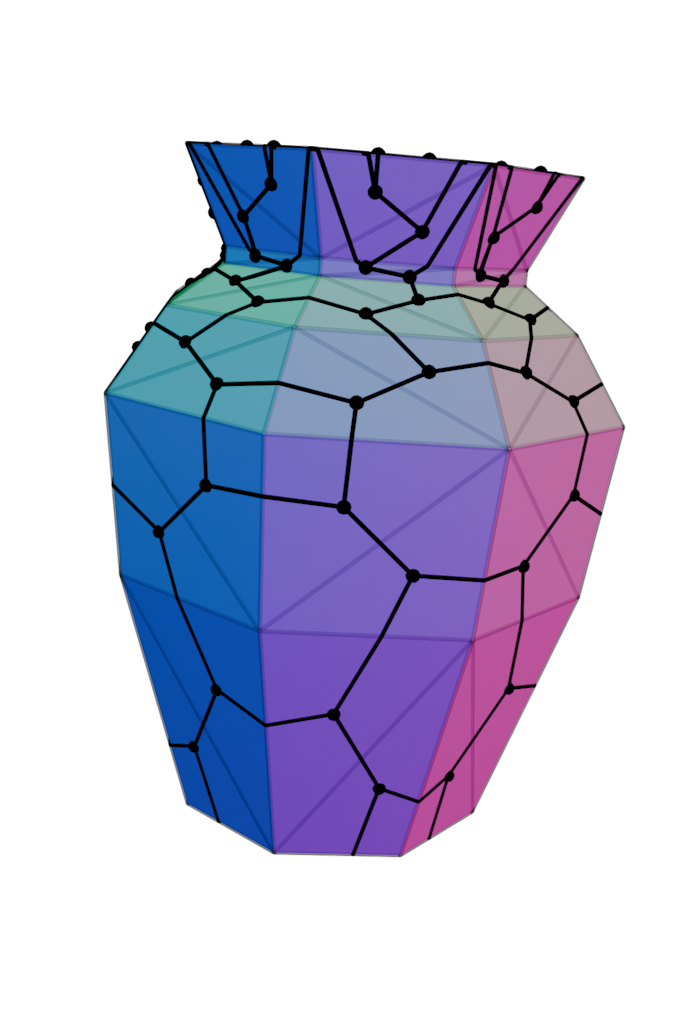
\includegraphics[width=0.25\textwidth]{figures/vase_dual.png}
        };
    \end{tikzpicture}
\end{wrapfigure}

In computer graphics, modeling, simulation, etc. we often want a representation of some real world geometry that we can perform computations on. A common way to of doing so is via a mesh. Consider the example mesh of a vase to the right. From some basic observations, the mesh appears to be comprised of points connected by segments/edges which outline faces. We formalize these observations in Definition \ref{def:tri_mesh}.

\begin{definition}
    \label{def:tri_mesh}
    A \term{triangular mesh} is a triple $K = (V, E, F)$ such that
    \begin{itemize}
        \item $V \subseteq \R^3$ is a finite set representing the vertices
        \item $E \subseteq [V]^2$ is a set representing non-intersecting edges
        \item $F \subseteq [E]^3$ is the set of faces such that for any $f = \qty{e_1, e_2, e_3} \in F$, we have $e_1 \cap e_2 = \qty{v_1}$, $e_2 \cap e_3 = \qty{v_2}$, and $e_3 \cap e_1 = \qty{v_3}$ for $v_1 \neq v_2 \neq v_3$. 
    \end{itemize}
\end{definition}

Notice that a triangular mesh lends itself to some very natural graph structures. One is simply using the vertices as the graph vertices and the edges as graph edges. The other one which is of use to us is using the faces as graph vertices and faces sharing a common edge as the edge set. This is often referred to as the dual graph of a mesh and appears in computational geometry problems such as mesh based signal processing \cite{taubinDualMeshResampling2002} and refinement of meshed implicit surfaces \cite{10.1145/566282.566308}. 

\begin{definition}
    The \term{dual mesh} of a triangular mesh $K = (V_K, E_K, F_K)$ is the graph $G = (V, E)$ such that $V = F_K$ and $f_1 \sim f_2$ if $f_1 \cap f_2 = \qty{e}$ for some in $e \in E_K$.
\end{definition}

\begin{theorem}
    A triangular mesh has $k$ connected components if and only the $0^\text{th}$ eigenvalue of the Laplacian matrix of its dual mesh has algebraic multiplicity $k$.
\end{theorem}

\newpage
\nocite{merrisLaplacianMatricesGraphs1994}
\printbibliography

\end{document}
